\documentclass{beamer}
\usetheme{Antibes}
\usecolortheme{orchid}
\usepackage{amsmath}
\usepackage[utf8]{inputenc}
\usepackage{tikz}
\usepackage{graphicx}
\usepackage{forest}
\usepackage{svg}

\usetikzlibrary{matrix}
\graphicspath{ {./} }

\usepackage{xcolor}

\definecolor{primary}{HTML}{0474E4}
\definecolor{secondary}{HTML}{2185D0}
\definecolor{tertiary}{HTML}{4183C4}
\definecolor{quaternary}{HTML}{384247}
\definecolor{magenta}{HTML}{FF00FF}

\setbeamercolor{palette primary}{bg=primary}
\setbeamercolor{palette secondary}{bg=secondary}
\setbeamercolor{palette tertiary}{bg=tertiary}
\setbeamercolor{palette quaternary}{bg=quaternary}

\setbeamercolor{block title}{fg=primary}
\setbeamercolor{local structure}{fg=primary}

\def\insertauthorindicator{Who?}% Default is "Who?"
\def\insertinstituteindicator{From?}% Default is "From?"
\def\insertdateindicator{When?}% Default is "When?"

\title{Approximate nearest neighbor search using the Hierarchical Navigable Small World (HNSW) algorithm}

\author{Sebastian Bj{\"o}rkqvist}
\institute{Lead AI Developer, IPRally}

\date[12.05.2023]{May 12, 2023}

\newcommand{\kur}{\protect\textit}
\newcommand{\bol}{\protect\textbf}
\newcommand\pro{\item[$+$]}
\newcommand\con{\item[$-$]}

\def\layersep{2.2cm}


\begin{document}
\setbeamertemplate{caption}{\raggedright\insertcaption\par}

\frame{\titlepage}


\begin{frame}
\frametitle{Outline}
  \tableofcontents
\end{frame}
\section{Theoretical foundations}
\subsection{Voronoi diagram}
  \begin{frame}
    \frametitle{Voronoi diagram for a set of points}  
  \begin{figure}[original_points]
    \vspace*{-0.1cm}
  	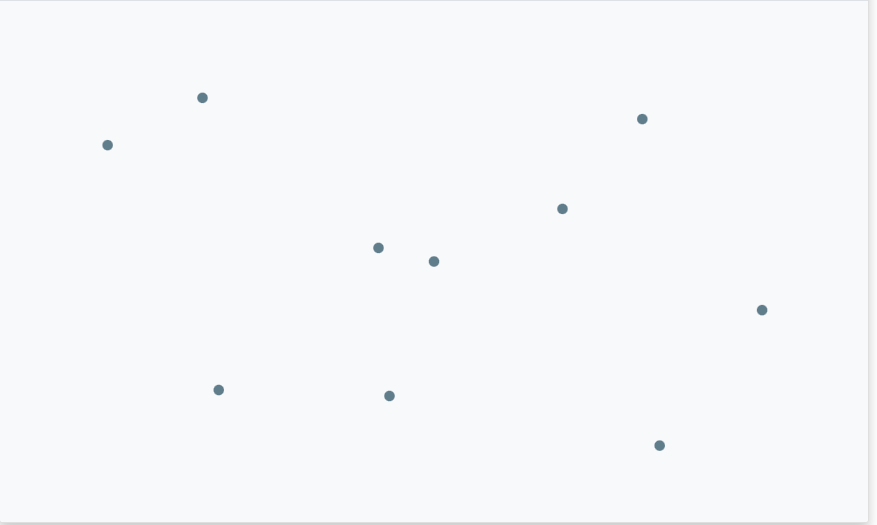
\includegraphics[scale=0.25]{original_points} 	
  \end{figure} 
  \end{frame}
  \begin{frame}
    \frametitle{Voronoi diagram for a set of points}  
  \begin{figure}[voronoi_diagram]
    \vspace*{-0.1cm}
  	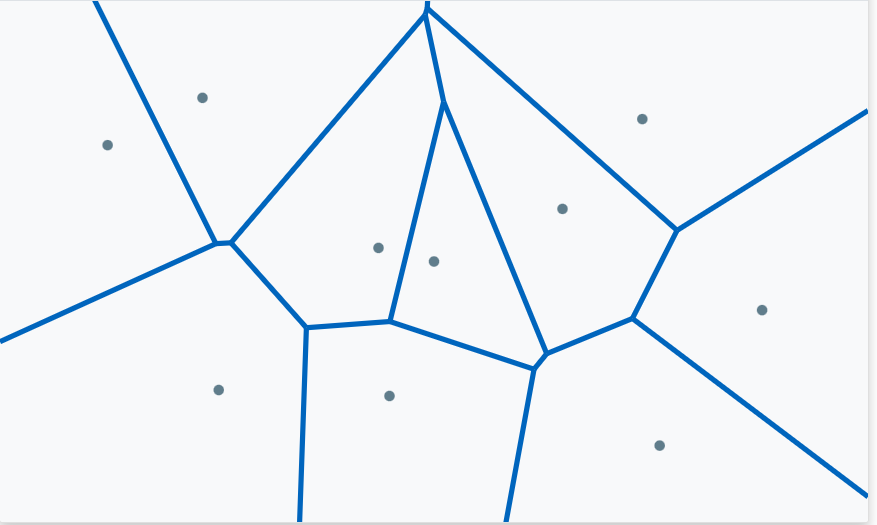
\includegraphics[scale=0.3]{voronoi_diagram} 	
  \end{figure} 
  \end{frame} 

\subsection{Delaunay graph}
  \begin{frame}
    \frametitle{Voronoi diagram to Delaunay graph}  
  \begin{figure}[voronoi_diagram]
    \vspace*{-0.1cm}
  	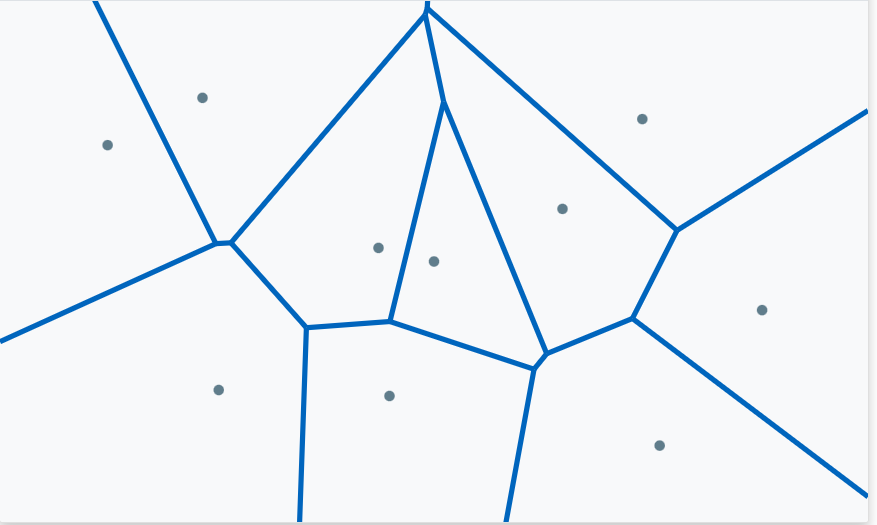
\includegraphics[scale=0.3]{voronoi_diagram} 	
  \end{figure} 
  \end{frame} 

  \begin{frame}
    \frametitle{Voronoi diagram to Delaunay graph}  
  \begin{figure}[voronoi_delaunay]
    \vspace*{-0.1cm}
  	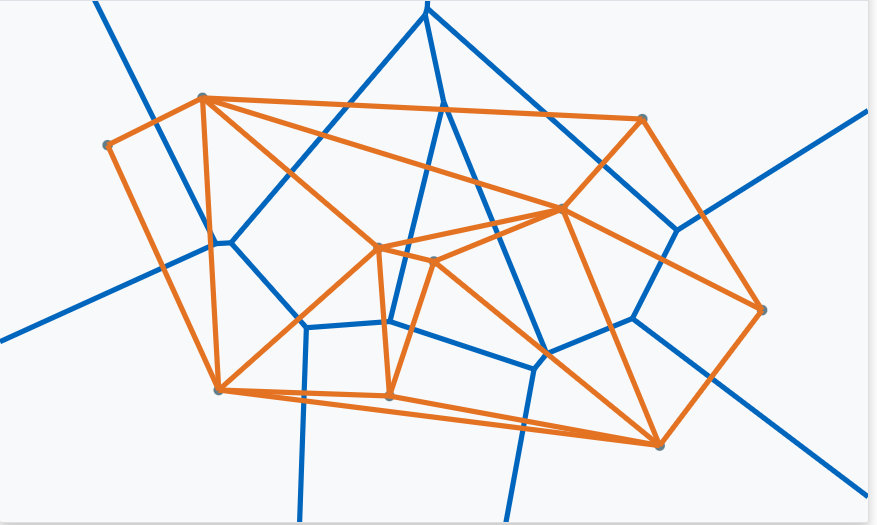
\includegraphics[scale=0.3]{voronoi_delaunay} 	
  \end{figure} 
  \end{frame} 

  \begin{frame}
    \frametitle{Delaunay graph}  
  \begin{figure}[delaunay_graph]
    \vspace*{-0.1cm}
  	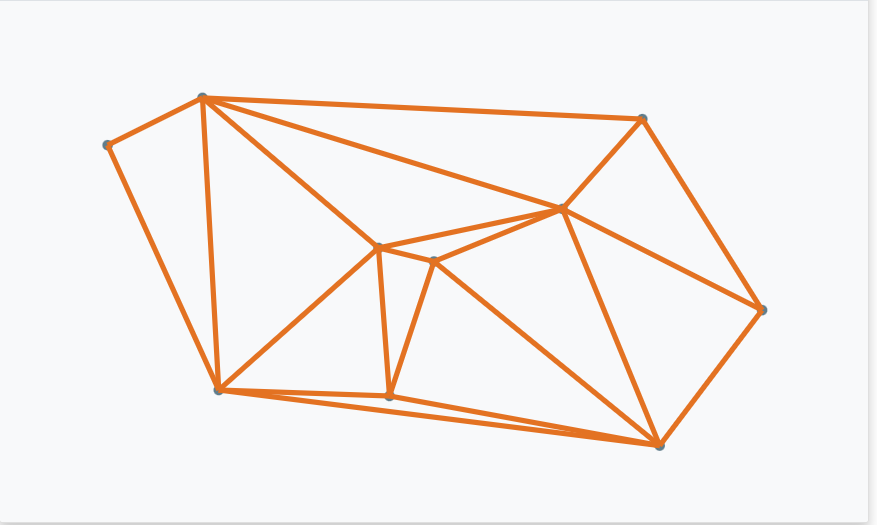
\includegraphics[scale=0.3]{delaunay_graph} 	
  \end{figure} 
  \end{frame} 
  
\subsection{Greedy NN search using Delaunay graph}

  \begin{frame}
    \frametitle{Greedy NN search algorithm}  
    \Large
   	\begin{enumerate}
   		\onslide<2->{
		\item Select any graph node as entry node}
		\onslide<3->{		
		\item Calculate distance from query to current node and from query to all neighbors of current node
		}
		\onslide<4->{
		\item Select neighbor with smallest distance to query as next node to visit
		}
		\onslide<5->{
		\item Repeat 2 and 3 until no neighbor is closer to query than the current node}
	\end{enumerate}  
  \end{frame}         
    

  \begin{frame}
    \frametitle{Greedy NN search start - Query and entry node}  
  \begin{figure}[greedy_search_start_new]
    \vspace*{-0.1cm}
  	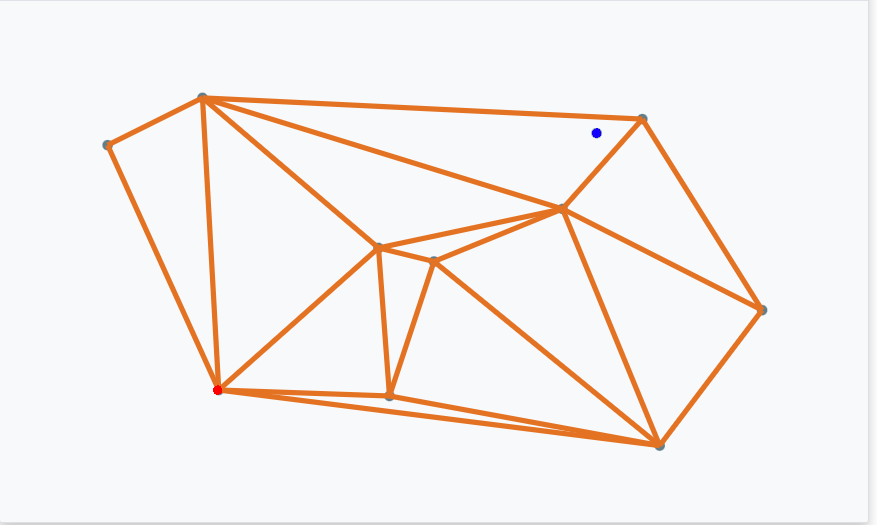
\includegraphics[scale=0.3]{greedy_search_start_new} 	
  \end{figure} 
  \end{frame} 
  

  \begin{frame}
    \frametitle{Greedy NN search - iteration}  
  \begin{figure}[greedy_search_start_new_step_1_1]
    \vspace*{-0.1cm}
  	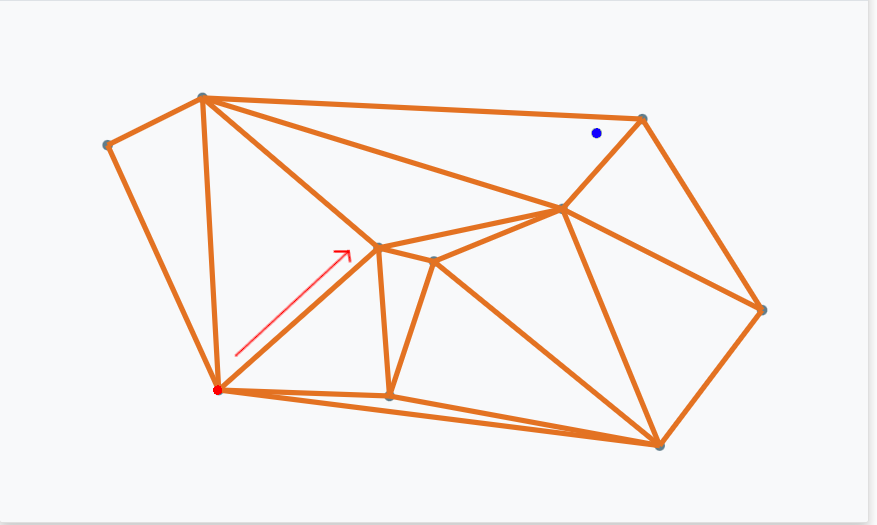
\includegraphics[scale=0.3]{greedy_search_start_new_step_1_1} 	
  \end{figure} 
  \end{frame}   
  

  \begin{frame}
    \frametitle{Greedy NN search - iteration}  
  \begin{figure}[greedy_search_start_new_step_1_2]
    \vspace*{-0.1cm}
  	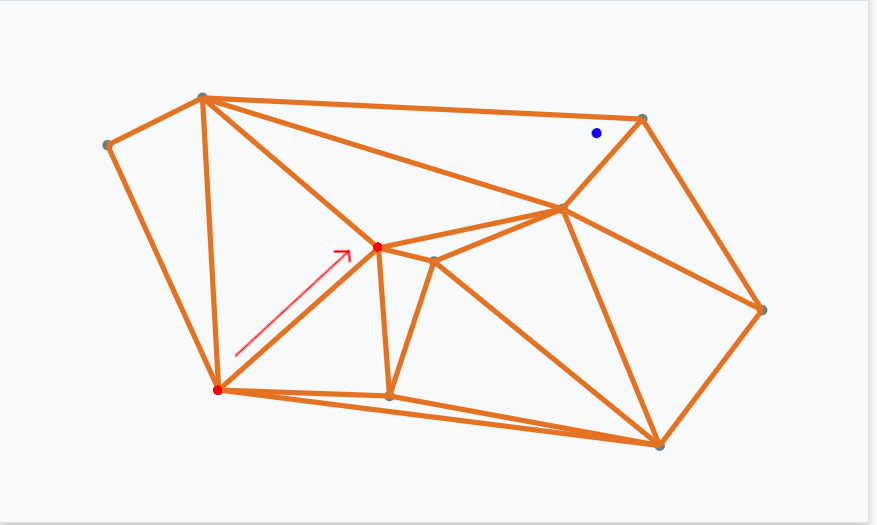
\includegraphics[scale=0.3]{greedy_search_start_new_step_1_2} 	
  \end{figure} 
  \end{frame}     
  

  \begin{frame}
    \frametitle{Greedy NN search - iteration}  
  \begin{figure}[greedy_search_start_new_step_2_1]
    \vspace*{-0.1cm}
  	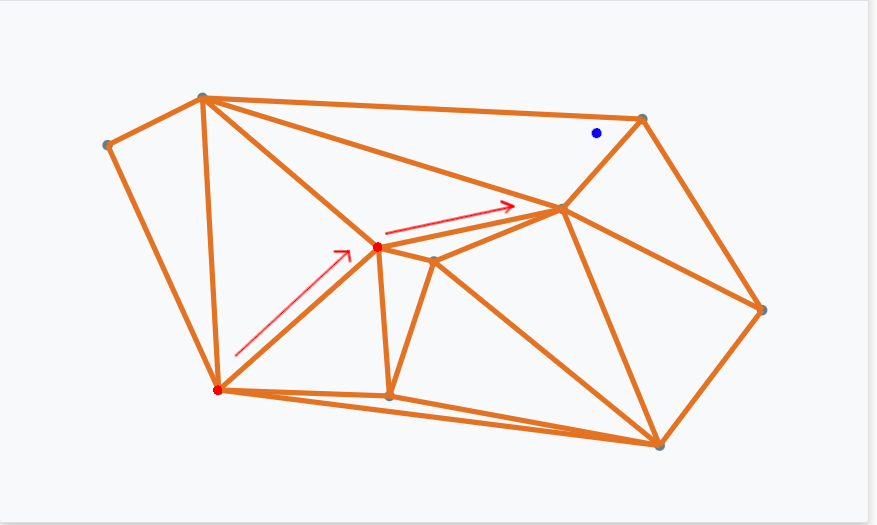
\includegraphics[scale=0.3]{greedy_search_start_new_step_2_1} 	
  \end{figure} 
  \end{frame}       
  
  \begin{frame}
    \frametitle{Greedy NN search - iteration}  
  \begin{figure}[greedy_search_start_new_step_2_2]
    \vspace*{-0.1cm}
  	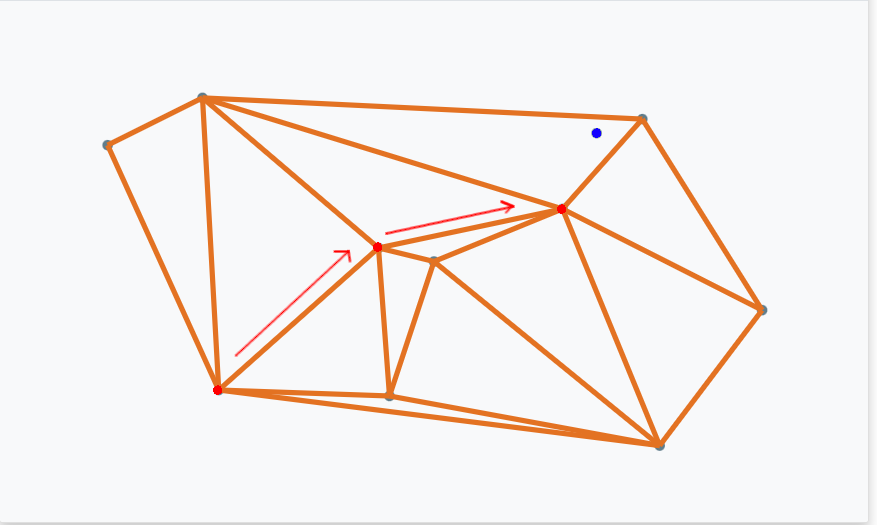
\includegraphics[scale=0.3]{greedy_search_start_new_step_2_2} 	
  \end{figure} 
  \end{frame}         

  \begin{frame}
    \frametitle{Greedy NN search - iteration}  
  \begin{figure}[greedy_search_start_new_step_3_1]
    \vspace*{-0.1cm}
  	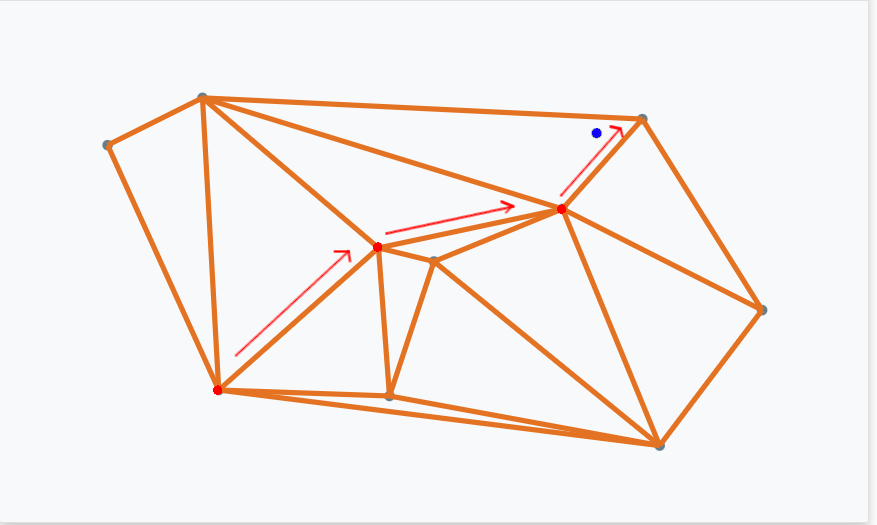
\includegraphics[scale=0.3]{greedy_search_start_new_step_3_1} 	
  \end{figure} 
  \end{frame}         


  \begin{frame}
    \frametitle{Greedy NN search done!}  
  \begin{figure}[greedy_search_start_new_step_3_2]
    \vspace*{-0.1cm}
  	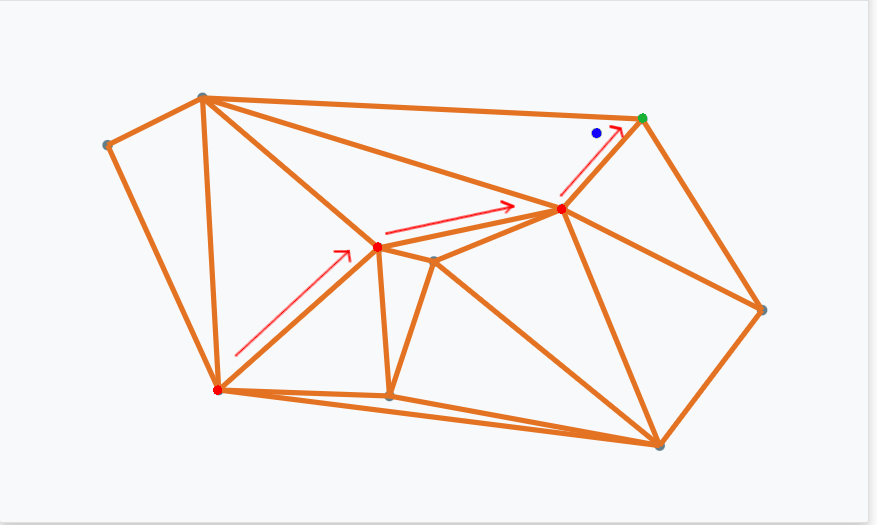
\includegraphics[scale=0.3]{greedy_search_start_new_step_3_2} 	
  \end{figure} 
  \end{frame}         
  

  \begin{frame}
    \frametitle{Drawbacks}  
   	\begin{itemize}
   	\Large
		\item Delaunay graph intractable to construct for large, high-dimensional data sets
		\item Greedy search might require a lot of steps if graph is large
	\end{itemize}   
  \end{frame}

\section{HNSW algorithm}
\subsection{Navigable small world (NSW)}
  \begin{frame}
    \frametitle{Navigable small world (NSW) graph}  
    \Large
   	\begin{itemize}
   		\onslide<2->{
		\item Small world graph}
		\begin{itemize}
		\onslide<3->{\item Distance of two random nodes is $log \text{ } N$, where $N$ is the number of nodes in graph}
		\onslide<4->{\item Neighbors of a given node are likely to be neighbors of another (clustering coefficient is high)}
		\end{itemize}
		\onslide<5->{		
		\item Navigability}
		\onslide<6->{
		\begin{itemize}
		\item Greedy search algorithm has logarithmic scalability
		\end{itemize}
		}
	\end{itemize}   
  \end{frame}

  \begin{frame}
    \frametitle{Why is an NSW useful for nearest neighbor search?}  
    \Large
    \begin{itemize}
    \onslide<2->{
    \item Logarithmic distance allows us to get anywhere in the graph quickly
    }
    \onslide<3->{
    \item Navigability ensures that the greedy algorithm finds the logaritmic path
    }
    \onslide<4->{
    \item High clustering coefficient lets us zoom in on the actual correct node when we're in the right area
    }
    \end{itemize}
  \end{frame}
  
  \begin{frame}
    \frametitle{Making Delaunay graph navigable}  
          \begin{figure}[delaunay_triangulation_256_points]
  \includesvg[scale=0.5]{delaunay_triangulation_256_points}
  \end{figure}
  \vspace{-0.5cm}
    \centering 256 nodes
  \end{frame}  

  \begin{frame}
    \frametitle{Making Delaunay graph navigable}  
          \begin{figure}[delaunay_triangulation_start_end_points]
  \includesvg[scale=0.5]{delaunay_triangulation_start_end_points}
  \end{figure}
  \end{frame}  

  \begin{frame}
    \frametitle{Making Delaunay graph navigable}  
          \begin{figure}[delaunay_triangulation_longest_path]
  \includesvg[scale=0.5]{delaunay_triangulation_longest_path}
  \end{figure}
  \vspace{-0.5cm}
    \centering Length of path: 19
  \end{frame}  

  \begin{frame}
    \frametitle{Making Delaunay graph navigable}  
          \begin{figure}[delaunay_triangulation_random_edges]
  \includesvg[scale=0.5]{delaunay_triangulation_random_edges}
  \end{figure}
  \vspace{-0.5cm}
    \centering 32 random edges added
  \end{frame}  

  \begin{frame}
    \frametitle{Making Delaunay graph navigable}  
          \begin{figure}[delaunay_triangulation_random_edges_shortest_path]
  \includesvg[scale=0.5]{delaunay_triangulation_random_edges_shortest_path}
  \end{figure}
  \vspace{-0.5cm}
    \centering Length of path: 5
  \end{frame}  


  \begin{frame}
    \frametitle{Properties of NSW graph}  
    \Large
    \onslide<2->{
    \begin{itemize}
    \item An NSW graph is not necessarily a Delaunay graph (or have one as a subgraph)
    }
    \onslide<3->{
    \item Thus the greedy algorithm doesn't always return the actual nearest neighbor
    }
    \onslide<4->{
    \item Ok since we're doing approximate nearest neighbor search!   
    }
    \end{itemize}
  \end{frame}
   

  \begin{frame}
    \frametitle{Constructing NSW graph}  
    \Large
   	\begin{itemize}
   		\onslide<2->{
		\item Goal: Construct a graph that has the Delaunay graph as a subgraph, but also has longer connections to make it navigable}
		\onslide<3->{		
		\item Approximation of Delaunay graph is sufficient
		}
	\end{itemize}   
  \end{frame}


  \begin{frame}
    \frametitle{Constructing NSW graph}  
    \Large
   	\begin{enumerate}
   		\onslide<2->{
		\item Randomize order of data points}
		\onslide<3->{		
		\item Add data point to graph
		}
		\onslide<4->{
		\item Add edges from data point to its $k$ nearest neighbors that are already present in the graph
		}
		\onslide<5->{
		\item Repeat 2 and 3 until all data points have been added}
	\end{enumerate}   
  \end{frame}


  \begin{frame}
    \frametitle{Why does NSW graph creation algorithm work?}  
    \Large
   	\begin{itemize}
   		\onslide<2->{
		\item Adding enough nearest neighbor edges approximates Delaunay graph}
		\onslide<3->{		
		\item The edges added for the early nodes give long-range connections, enabling navigability
		}
	\end{itemize}   
  \end{frame}

  \begin{frame}
    \frametitle{kNN search using NSW graph}  
    \Large
   	\begin{itemize}
   		\onslide<2->{
		\item Instead of only finding the nearest neighbor, we keep track of $k$ nearest neighbors}
		\onslide<3->{		
		\item To improve results we can redo the search $m$ times from different start nodes
		}
	\end{itemize}   
  \end{frame}

  \begin{frame}
    \frametitle{kNN search algorithm}  
   	\begin{enumerate}

   		\onslide<2->{
		\item Select any graph node as initial candidate, initialize candidates priority queue with initial candidate, initialize empty result priority queue}
		\onslide<3->{		
		\item Select from the candidates queue the element closest to q	
		}
		\onslide<4->{		
		\item Calculate distance from query to all neighbors of candidate
		}
		\onslide<5->{
		\item Add to result set and to candidate queue all neighbors who are closer to query than the kth result in the queue
		}
		\onslide<6->{
		\item Repeat until step 2 returns a candidate that's further away than the kth result in the queue} 
	\end{enumerate} 
  \end{frame}

  \begin{frame}
    \frametitle{NSW drawbacks}  
    \Large
   	\begin{itemize}
   		\onslide<2->{
		\item Greedy search may get stuck in local minimum}
		\onslide<3->{		
		\item Algorithm scales polylogarithmically in general (logarithmic scaling in both steps and degrees of nodes)
		}
		\onslide<4->{		
		\item Performance degrades on high-dimensional data
		}
		\onslide<5->{		
		\item Insertion order must be random
		}
	\end{itemize}   
  \end{frame}


\subsection{Hierarchical navigable small world (HNSW)}

\begin{frame}
\frametitle{Inspiration: Skiplist}
          \begin{figure}[skip_list]
  \includesvg[scale=0.9]{skip_list}
  \end{figure}
  \vspace{-0.1cm}
  \small \centering \url{https://en.wikipedia.org/wiki/Skip_list}
\end{frame}

\begin{frame}
\frametitle{Idea: Combine NSW and skipping}
    \Large
   	\begin{itemize}
   		\onslide<2->{
		\item NSW enables finding the approximate nearest neighbors}
		\onslide<3->{		
		\item Skipping allows zooming in to the correct area quickly and reliably 
		}
		\onslide<4->{		
		\item The zoom-in property is accomplished by a hierarchical construction, like in skiplists
		}
	\end{itemize} 
\end{frame}

  \begin{frame}
    \frametitle{HNSW diagram}  
  \begin{figure}[hnsw_paper_fig_1]
    \vspace*{-0.1cm}
  	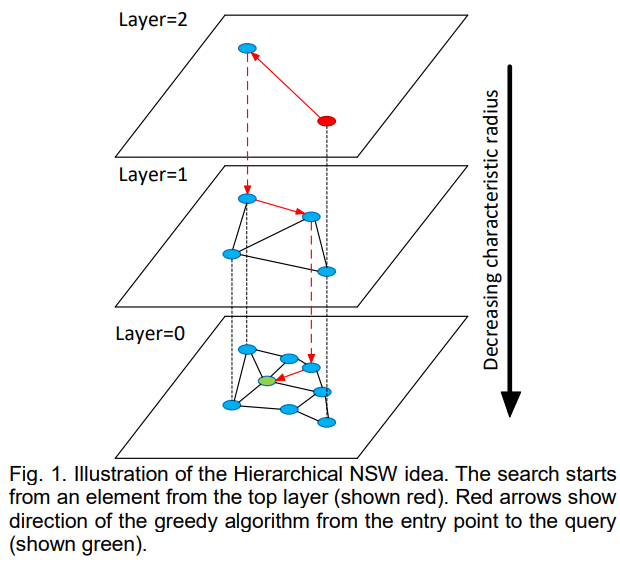
\includegraphics[scale=0.3]{hnsw_paper_fig_1} 	
  \end{figure} 
  \vspace{-0.3cm}
  \scriptsize \centering \textit{Efficient and robust approximate nearest neighbor search using Hierarchical Navigable Small World graphs (Malkov et al.)} \url{https://arxiv.org/abs/1603.09320} 
  \end{frame}

  \begin{frame}
    \frametitle{kNN search using HNSW}  
   	\begin{enumerate}

   		\onslide<2->{
		\item Find nearest neighbor to query in top layer using greedy search algorithm, starting from any node}
		\onslide<3->{		
		\item Continue downwards to next layer, run greedy search starting from nearest neighbor found in previous layer}
		\onslide<4->{		
		\item Repeat previous step until bottom layer is reached
		}
		\onslide<5->{
		\item Run kNN algorithm on bottom layer (like when using NSW)}
	\end{enumerate} 
  \end{frame}
  
\subsection{Nearest neighbor search using HNSW}

  \section{Performance}
\subsection{Search accuracy}




\subsection{Build time}

\section{}
  \begin{frame}
    \frametitle{References}  
    \small
    \begin{itemize}
	\item \textit{Efficient and robust approximate nearest neighbor search using Hierarchical Navigable Small World graphs (Malkov et al.)} \url{https://arxiv.org/abs/1603.09320}    

	\item \textit{Approximate nearest neighbor algorithm based on navigable small world graphs (Malkov et al.)} \url{https://doi.org/10.1016/j.is.2013.10.006}	
	\item \textit{Voronoi diagrams—a survey of a fundamental geometric data structure (Aurenhammer)} \url{https://dl.acm.org/doi/10.1145/116873.116880}
	\item \textit{Hierarchical Navigable Small Worlds (HNSW) (Pinecone blog)} \url{https://www.pinecone.io/learn/hnsw/}
	\end{itemize}
	
  \end{frame}



\end{document}
